\documentclass[runningheads,a4paper]{llncs}
\usepackage[utf8]{inputenc}
\usepackage[T1]{fontenc}
\usepackage{csquotes}
\usepackage[english]{babel}
\usepackage[backend=bibtex,natbib,hyperref=true,maxnames=2,style=authoryear-comp]{biblatex}
\addbibresource{seminarreport.bib}

\usepackage{amsmath}
\usepackage{booktabs}
\usepackage{enumitem}
\usepackage{graphicx}
\usepackage{eurosym}
\usepackage[hidelinks]{hyperref}
\usepackage[capitalise]{cleveref}

\DeclareMathOperator*{\somefunc}{somefunc}
%
\begin{document}
%
\frontmatter          % for the preliminaries
%
\pagestyle{headings}  % switches on printing of running heads
%
\mainmatter              % start of the contributions
%
\title{Your Topic}
\subtitle{Seminar/Lab Title}
%
\titlerunning{Lab Title (again!)}  % abbreviated title (for running head)
%
\author{Last Name, First Name}
%
\authorrunning{Last name, first name}   % abbreviated author list (for running head)
\institute{Universit\"at Bonn\\
\email{EMAIL@cs.uni-bonn.de},
Matrikelnummer: XXXXXX
}

\maketitle              % typeset the title of the contribution

\begin{abstract}
    This is  the abstract. It summarizes your  contribution. It should only
    have one paragraph, but very briefly summarize everything in your document.
\end{abstract}

\section{Introduction}

\subsection{Paragraphs}
\label{sec:paras}

Paragraphs are separated  by empty lines in the  \LaTeX{} code.  Never 
use  the double  backslash for  this purpose.   \LaTeX{} inserts  page 
breaks  preferably between  paragraphs.  A  double backslash  lets you 
stay in the  same paragraph, so \LaTeX{} does not  know where it would 
be good  to insert page  breaks, figures, tables, algorithms,  and the 
like.                                                                  

Many  people find  the  indentation  of the  first  line in  paragraph 
odd.  Look into  a favorite book or newspaper of  yours and you'll see 
that this way of introducing  new paragraphs is used everywhere.  Note 
that it  allows you---even on the  top of a new  page---to see whether 
the line is the first of a new paragraph or the continuation of an old 
paragraph.                                                             

\subsection{Typesetting Math as Part of Your Text}

Formulas are part of the text, try  to use them like nouns and be sure 
to include  punctuation to  keep the text  flowing.  For  example, the 
pythagorean theorem,                                                   
\begin{align}
    a^2 + b^2 = c^2,
\end{align}
is typically taught at school.

Other random notes:

\begin{itemize}
    \item
Note that  as in \cref{sec:paras},  before and after a  formula, empty 
lines will  add space  and indentation, and  possibly page  breaks, or 
figures.  So  if a formula  is part of a  paragraph, do not  add empty 
lines around it in the code.                                           

    \item
Number all equations.  It makes it  easier to refer to them for others,
even if you do not refer to them in your own text.

    \item
While we're at  it, do not use the  \verb+equation+ or \verb+eqnarray+ 
environments, use \verb+align+ instead.

    \item
Take care to always put all  math in the math-environment, for example 
the  variable $x$.   Note  that  it is  typeset  differently from  the 
letter~x.

    \item
Use  single-letter  names  for  variables   in  math  (math  is  not  a
programming language!).   Function names  may have  multiple characters,
such as $\tanh(x)$.  Note that they are not typeset in italics.  
They  usually have  their own  commands, and  you can  define your  own
functions, such as  $\somefunc(x)$.  If you don't do  this, the kerning
will  be broken,  since \LaTeX{}  assumes that  you're multiplying  the
variables  $s$, $o$,  $m$, $e$,  $f$, $u$,  $n$, and  $c$ and  typesets
accordingly,  compare  $somefunc$  (math  mode,  without  spaces!)  and
\emph{somefunc} (italics).

\end{itemize}

\subsection{Citing other works}

The  works you  want to  reference go  in the  file \verb+report.bib+. The 
\verb+\printbibliography+ command generates the references list at the end 
of this document.  In  the main text, you cite the keys  of the entries in 
your bib file. This ensures consistency of content and style.

There are two ways to cite, which depends on whether the authors are an
active part of your sentence:
\begin{itemize}[noitemsep]
    \item \citet{Bailey} showed that\ldots{}
    \item This is currently a hot research topic \citep{Bailey}
\end{itemize}
In  \LaTeX{}, these  different  citation styles  are  reflected in  the
\texttt{\textbackslash citet}  and  \texttt{\textbackslash citep}  commands. 
\textit{Never  use  the  plain
\texttt{\textbackslash cite}!} -- it is outdated.
This distinction  is even more important  when you use a  numeric style
for referencing, where in the second version only the number of the 
reference is printed.   In the first case, a  number-only citation does
not make much sense.

\subsection{Quotes}
Note that double "quotes" on  your keyboard are not typeset correctly. 
English  quotes should  look like  ``this'', while  German quotes  are 
typeset  like \glqq this\grqq.   Note the  difference.  Some  editors 
insert the correct quotes automatically for you.                       

\subsection{Emphasis and Line Noise}
Use  emphasis  sparingly.  It  clutters  the  text.  In  general,  use 
\emph{italics}, which is the one standing out the least.  In captions, 
it is sometimes useful to use  \textbf{bold} for the signal words left 
and right, top and bottom: There, you want them to pop out.

Do  not use  fill words  which do  not carry  meaning.  Try  to be  as 
specific as  possible.  This does  not mean  as short as  possible, it 
means that you should have something to say when you write something.
If you don't know what you want to say, think again, \emph{then} write.

Don't use colloquial expressions.  In particular, don't use any of the 
short forms  \emph{don't, aren't,  isn't, you're, we're,  \ldots}.  Do 
not\footnote{this is much better!} use  ellipsis (\ldots) in the text, 
as it looks like you're trailing off.                                  

\subsection{Compiling the Document}
\LaTeX{}  is  a bit  archaic  to  work  with,  since with  every  pass 
through  your document,  some intermediate  information is  written to 
files,  which are  then processed  by  other programs.   Keep in  mind 
that  every time a  new  pass through  your  document incorporates  new 
information (e.g. from BibTeX), page breaks may change, which requires
an  additional pass  through the  document. Thus, you  usually have  to
compile the document in three steps:
\begin{enumerate}
    \item Compile the document using xelatex: xelatex thesis
    \item Run biber  (or if  you do  not have  it, bibtex)  to set  up
          bibliography: biber thesis
    \item Run xelatex  twice more to incorporate  bibtex references and
          to get the typesetting right.
\end{enumerate}


\begin{figure}[tbp]
    \centering
    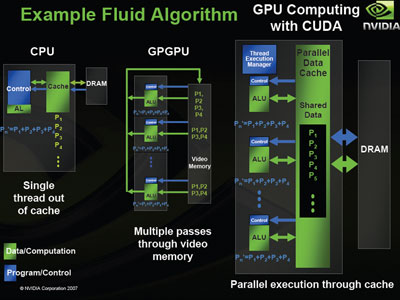
\includegraphics[width=.5\linewidth]{pic/cuda.jpg}
    \caption{Something about CUDA architecture. Quite interesting.}
    \label{fig:cuda}
\end{figure}

If  you know  what  you're doing  you  can get  away  with less.   Some
programs parse the  output of \LaTeX{} to  determine whether additional
passes are necessary.  Most GUI programs fall in this category, as do
\verb+rubber+ and \verb+latexmk+.

\section{Related Work}


\section{Methods}


\section{Results}

    \begin{table}
        \centering
        \begin{tabular}{@{}lrr@{}} 
            \toprule
            \multicolumn{2}{c}{Education}\\ \cmidrule{1-2}
            Major & Duration & Income (\euro)\\ 
            \midrule 
            CompSci & 2 & 12,75 \\ \addlinespace
            MST & 6 & 8,20 \\ \addlinespace
            VWL & 14 & 10,00\\ 
            \bottomrule
        \end{tabular}
        \caption[Table Example]{A basic example from the booktabs package.}
        \label{tab::ex}
    \end{table}

Tables  and  figures are  put  in  floats.  They  usually float  to  the
top  of  the  page,  and  you  reference them  from  the  main  text  using
\verb+\cref{tab::ex}+, displayed as \cref{tab::ex}.

Do  not use  vertical  lines  in tables,  see  the \verb+booktabs+  package
documentation for explanation and examples.

All tables and  figures have a caption from which  you can understand most 
of the  content and its significance.   They are also referenced  from the 
main  text  (e.g.,  see  \cref{fig:cuda}).  Do  not  force  linebreaks  in 
captions.  


\section{Conclusion}

\printbibliography
\end{document}
